% In preamble:
% \usepackage{pgfplots}
% \pgfplotsset{compat=1.18}

\begin{figure}[h!]
\centering
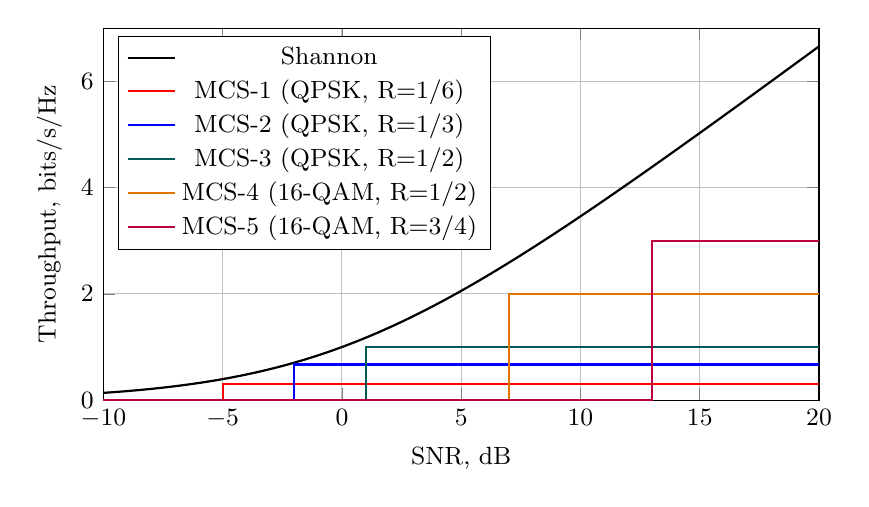
\begin{tikzpicture}
\begin{axis}[
    width=0.88\textwidth,
    height=0.52\textwidth,
    xlabel={SNR, dB},
    ylabel={Throughput, bits/s/Hz},
    xmin=-10, xmax=20,
    ymin=0, ymax=7,
    grid=both,
    major grid style={gray!50},
    minor grid style={gray!20},
    legend style={
        at={(0.02,0.98)},
        anchor=north west,
        fill=white,
        draw=black,
        font=\small
    },
    tick label style={font=\small},
    label style={font=\small},
    every axis plot/.append style={thick}
]

% Shannon
\addplot[domain=-10:20,samples=300,black]
    {ln(1 + 10^(x/10))/ln(2)};
\addlegendentry{Shannon}

% Simple step-like MCS curves
\addplot[red, const plot]
coordinates {
(-10,0) (-5,0) (-5,0.30) (20,0.30)
};
\addlegendentry{MCS-1 (QPSK, R=1/6)}

\addplot[blue, const plot]
coordinates {
(-10,0) (-2,0) (-2,0.67) (20,0.67)
};
\addlegendentry{MCS-2 (QPSK, R=1/3)}

\addplot[teal!70!black, const plot]
coordinates {
(-10,0) (1,0) (1,1.00) (20,1.00)
};
\addlegendentry{MCS-3 (QPSK, R=1/2)}

\addplot[orange!90!black, const plot]
coordinates {
(-10,0) (7,0) (7,2.00) (20,2.00)
};
\addlegendentry{MCS-4 (16-QAM, R=1/2)}

\addplot[purple, const plot]
coordinates {
(-10,0) (13,0) (13,3.00) (20,3.00)
};
\addlegendentry{MCS-5 (16-QAM, R=3/4)}

\end{axis}
\end{tikzpicture}
\caption{Modulation and coding throughput versus SNR.}
\label{fig:amc_snr}
\end{figure}